%!TEX program = lualatex
% SPDX-License-Identifier: CC-BY-SA-4.0
\documentclass[11pt]{article}

\usepackage{iftex}
\ifLuaTeX\else
  \PackageError{vintage-latex}{This example requires LuaLaTeX}
    {Run lualatex, not pdflatex or xelatex.}
\fi

\usepackage{fontspec}
\usepackage{xcolor}
\usepackage{geometry}
\usepackage{tikz}
\usetikzlibrary{decorations.pathmorphing,patterns.meta}

\setmainfont{EB Garamond}[Ligatures={TeX,Common,Rare}]
\definecolor{ragpaper}{HTML}{F4EBDD}
\definecolor{printerink}{HTML}{231F1A}
\pagecolor{ragpaper}
\color{printerink}
\geometry{a4paper,margin=28mm}
\pagestyle{empty}

\tikzset{
  etched/.style={
    draw=printerink,
    line width=0.58pt,
    line cap=round,
    line join=round,
    decorate,
    decoration={random steps,segment length=2.7pt,amplitude=0.16pt}
  },
  fine etched/.style={
    etched,
    line width=0.38pt,
    decoration={random steps,segment length=2.2pt,amplitude=0.11pt}
  },
  single hatch/.style={
    pattern={Lines[angle=58,distance=3.2pt,line width=0.28pt]},
    pattern color=printerink
  },
  cross hatch/.style={
    pattern={Hatch[distance=3.4pt,xshift=0pt,yshift=0pt,
                   line width=0.24pt]},
    pattern color=printerink
  }
}

\begin{document}

\begin{center}
  {\Large\textsc{Plate I}}\\[0.35em]
  {\small\textit{A monochrome scheme of refraction}}\par
\end{center}

\vspace{1.1em}

\begin{center}
\pgfmathsetseed{1729}% makes the irregular strokes reproducible
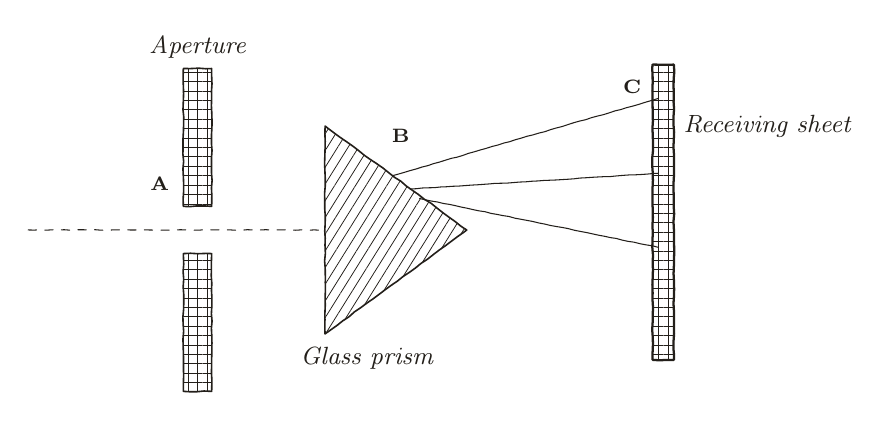
\begin{tikzpicture}[x=1cm,y=1cm]
  % Dark-room screen and slit.
  \path[cross hatch] (-0.18,-2.05) rectangle (0.18,-0.30);
  \path[cross hatch] (-0.18, 0.30) rectangle (0.18, 2.05);
  \draw[etched] (-0.18,-2.05) rectangle (0.18,-0.30);
  \draw[etched] (-0.18, 0.30) rectangle (0.18, 2.05);
  \node[above,font=\small\itshape,text=printerink] at (0,2.05) {Aperture};

  % Incident beam. The clear gap in the screen remains measurable.
  \draw[fine etched,dashed] (-2.15,0) -- (1.62,0);

  % Hatched glass body, followed by a separately jittered outline. Separating
  % fill from outline prevents the decoration from mangling the hatch clip.
  \path[single hatch] (1.62,-1.32) -- (3.42,0) -- (1.62,1.32) -- cycle;
  \draw[etched] (1.62,-1.32) -- (3.42,0) -- (1.62,1.32) -- cycle;
  \node[font=\small\itshape,text=printerink] at (2.15,-1.63) {Glass prism};

  % A monochrome fan of refracted rays.
  \draw[fine etched] (2.48, 0.69) -- (5.85, 1.67);
  \draw[fine etched] (2.70, 0.52) -- (5.85, 0.72);
  \draw[fine etched] (2.82, 0.40) -- (5.85,-0.22);

  % Receiving sheet with two-direction hatch behind the outline.
  \path[cross hatch] (5.78,-1.65) rectangle (6.05,2.10);
  \draw[etched,line width=0.82pt] (5.78,-1.65) rectangle (6.05,2.10);
  \node[right,font=\small\itshape,text=printerink] at (6.05,1.32)
    {Receiving sheet};

  % Lettered callouts remain text in the PDF.
  \node[font=\scriptsize\bfseries,text=printerink] at (-0.48,0.58) {A};
  \node[font=\scriptsize\bfseries,text=printerink] at (2.58,1.20) {B};
  \node[font=\scriptsize\bfseries,text=printerink] at (5.52,1.82) {C};
\end{tikzpicture}
\end{center}

\vspace{1.2em}

\begin{center}
  \small\itshape
  Fig. 1. The line irregularity is seeded; the hatched fields remain regular
  enough to describe material and shadow without gray fills.
\end{center}

\vfill
\noindent\footnotesize
The construction deliberately uses separate paths for hatching and outlines.
This keeps the physical roles legible: patterns indicate tone or material,
while the restrained random-step decoration affects only the drawn contour.

\end{document}
